\documentclass[11pt,a4paper]{article}

\usepackage{graphicx}
\usepackage{float}
\usepackage{amsmath}
\usepackage{url}
\usepackage{listings}
\usepackage[a4paper,left=3cm,right=2cm,top=2.5cm,bottom=2.5cm]{geometry}


\renewcommand{\baselinestretch}{1.5}
\everymath{\displaystyle}
\date{}

\title{Clustering majors by socio-economic characteristics}

\begin{document}
\newpage
\maketitle

\section*{Introduction}

\begin{itemize}
    \item Every high school student that is willing to pursue a higher education degree has to answer a burning question about his future education "What major am I going to select ?".
    \item Majors are grouped together into 16 existing major categories such as engineering, law, education, etc. based on the area of study and topic.
    \item While clustering the majors based on topic might help a student first pick a major category and narrow down their choices, it would be useful to know if majors can be clustered together using socio-economical properties such as income, gender distribution and employment rate.
    \item This clustering  would allow us to answer questions such as "Which group of majors has the highest median income but share similar socio-economic characteristics?" or "Which group of major has the highest number of full-employed students ?".
    \item For a student, this sort of clustering would allow focusing on major clusters that are actually offering good life prospects, and would allow picking between different topics that have similar vocational perspectives.
    \item For governments and universities, this clustering would allow the discovery of obsolete degrees or degrees that are not attractive because the job market is supersaturated, or the demand has decreased, and replace them with more attractive ones.
    \item Ultimately, it would be interesting to know how big is the overlap between the clustering done based on socio-economic properties and the current grouping based on topic. 
\end{itemize}

\section*{Methods}

\begin{itemize}
    \item The dataset contains 172 observations and 17 numerical variables. A big majority of the variables have a high correlation between them. Only one of the majors contains empty values, which will be removed from the analysis.
    \item Given that the variables are on different scales, these will be scaled and centered before applying the analysis
    \item Before applying clustering, PCA will be performed to retain the components with the highest variance and reduce the dimensions. To select the number of dimensions, will use scree plots and plot the cumulative explained variance vs dimension. Given that the numerical variables have a high correlation, the expectation is that PCA will reduce the dimension from 17 numerical variables to about 2-3 while also explain 80-90\% of variance.
    \item Run k-means clustering with variable number of clusters. As with PCA, use scree plots to consider what is the optimal number of cluster that reduces the within-group SSE. Additionally, use silhouette plots to check how well majors are classified.
    \item Analyze the clusters and check the overlap with the 16 existing major categories available, and compute a measure of cluster purity, by considering how many major categories are part of the same cluster.
    \item Make plots and summaries to draw conclusion 
\end{itemize}

\begin{figure} [H]
    \begin{center}
        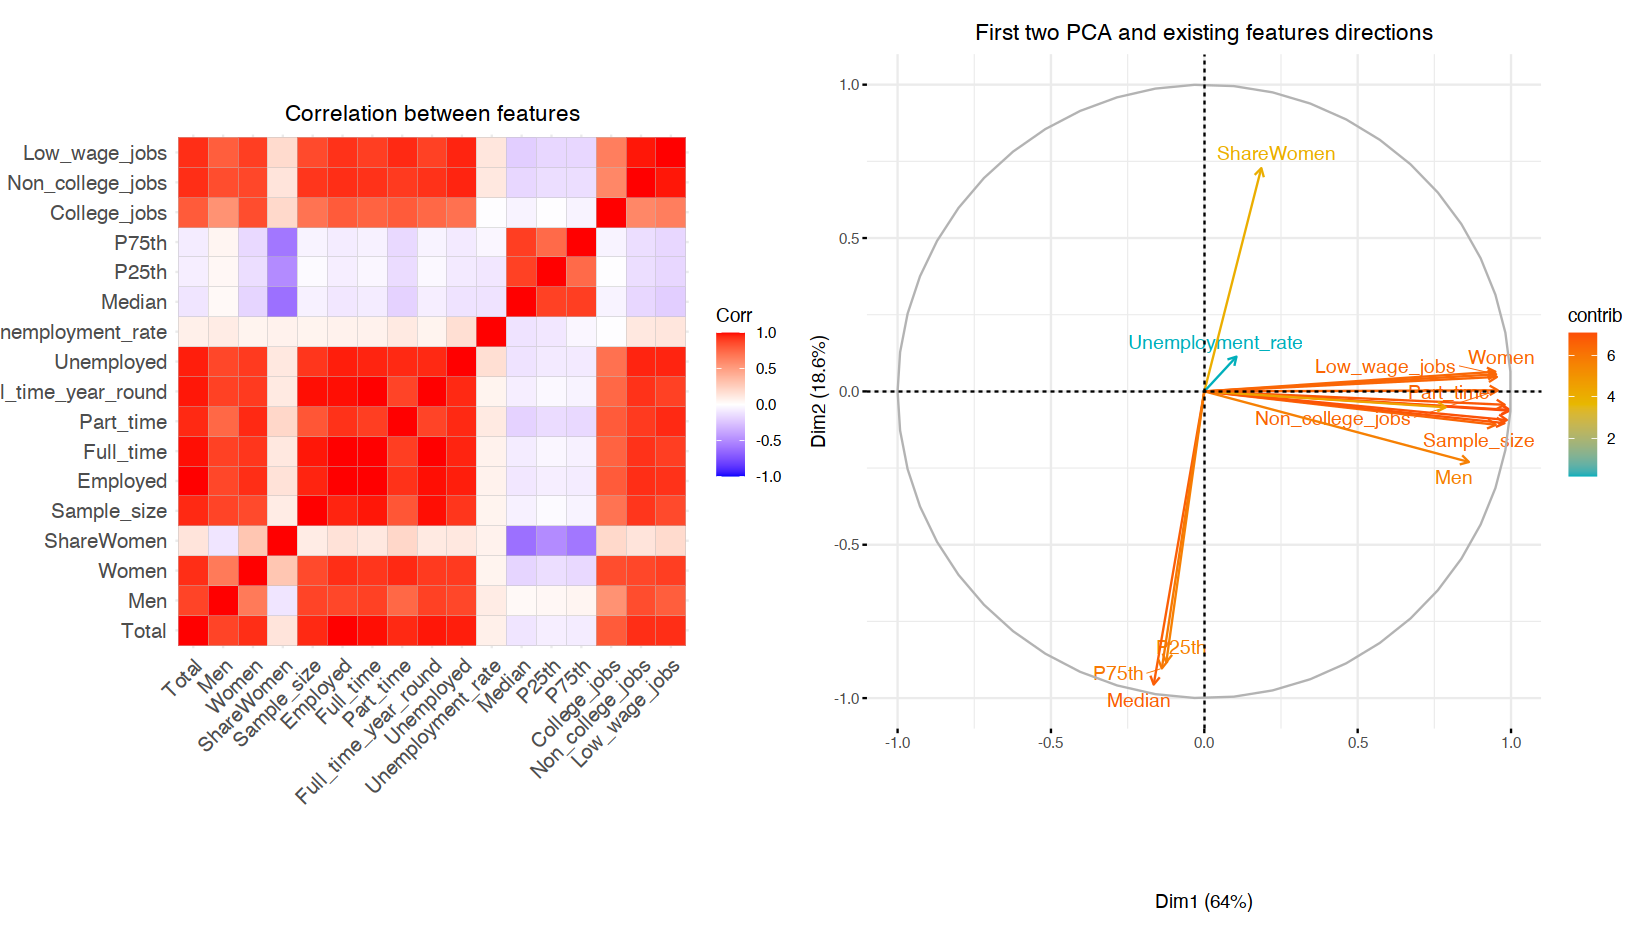
\includegraphics[scale=1, width=18cm]{plots.png}
        \label{fig:sampledvsdata}
    \end{center}
\end{figure}



\end{document}\models